% ============================================================
%  Artificial Intelligence: A Textbook
%  Chapter 2 — Searching State Spaces
%  Offline Beamer slides (uses shared theme.tex + branding.tex)
%  Prince Sattam Bin Abdulaziz University — CCES
% ============================================================
\documentclass[aspectratio=169,11pt]{beamer}

\input{theme.tex}

% ---------- COURSE RE-BRANDING (AI instead of CS3401) --------
\graphicspath{{../chapters/images/ch2/}{../chapters/images/}}
\input{branding.tex}
\usetikzlibrary{quotes}

% ---------- SLIDE METADATA ----------------------------------
\title[Ch.\,2 — Search]{Searching State Spaces}
\subtitle{Chapter 2 — Uninformed, Informed, and Local Search}
\author{Dr.\ Khalil Chebil}
\date{Artificial Intelligence Course}

% Inline check / cross marks
\newcommand{\cmark}{\textcolor{SuccessGreen}{\ensuremath{\checkmark}}}
\newcommand{\xmark}{\textcolor{AlertRed}{\ensuremath{\times}}}

\begin{document}

% ============================================================
%  TITLE
% ============================================================
{\setbeamertemplate{footline}{}
\begin{frame}[plain,noframenumbering]
  \titlepage
\end{frame}}

% ============================================================
%  OUTLINE
% ============================================================
\begin{frame}{Chapter Outline}{What we will cover}
  \begin{columns}[T]
    \begin{column}{0.5\textwidth}
      \tableofcontents[sections={1-3}]
    \end{column}
    \begin{column}{0.5\textwidth}
      \tableofcontents[sections={4-5}]
    \end{column}
  \end{columns}
  \vfill
  \begin{block}{Learning Objectives}
    \begin{itemize}
      \item Represent problems as \keyword{state-space graphs}
      \item Master \keyword{uninformed} search: BFS, DFS, UCS, bidirectional
      \item Master \keyword{informed} search: greedy best-first and A$^\ast$
      \item Design \keyword{admissible} heuristics; apply \keyword{local search} and \keyword{genetic algorithms}
    \end{itemize}
  \end{block}
\end{frame}

% ============================================================
\section{Search Problems \& State Spaces}
% ============================================================

\begin{frame}{What is Search?}{Finding a path from start to goal}
  \begin{columns}[T]
    \begin{column}{0.54\textwidth}
      Many AI problems reduce to finding a \keyword{sequence of actions}
      transforming an \keyword{initial state} into a \keyword{goal state}.
      \vspace{0.4em}
      \begin{block}{Two scenarios}
        \small
        \begin{itemize}
          \item \keyword{Goal-oriented}: find a path (maze, puzzle)
          \item \keyword{Optimization}: find a best state (8-queens, scheduling)
        \end{itemize}
      \end{block}
    \end{column}
    \begin{column}{0.46\textwidth}
      \begin{exampleblock}{Why search matters}
        \small
        \begin{itemize}
          \item No closed-form solution
          \item Huge solution spaces
          \item Needs systematic exploration
          \item Trades time, memory, quality
        \end{itemize}
      \end{exampleblock}
    \end{column}
  \end{columns}
  \vspace{0.3em}
  \begin{center}\scriptsize
    Applications: route planning \textbullet\ puzzles \textbullet\ game playing
    \textbullet\ scheduling \textbullet\ robot navigation
  \end{center}
\end{frame}

\begin{frame}{State Space as a Graph}{Nodes, edges, paths}
  \begin{columns}[c]
    \begin{column}{0.5\textwidth}
      \begin{itemize}
        \item \keyword{Node} — a state
        \item \keyword{Edge} — an action / transition
        \item \keyword{Path} — sequence from start to goal
      \end{itemize}
      \vspace{0.3em}
      \begin{block}{State-space size explodes}
        \scriptsize
        \begin{tabular}{@{}ll@{}}
          8-Puzzle & $9! = 362{,}880$ \\
          8-Queens & ${64 \choose 8}\approx 4.4\times10^{8}$ \\
          Rubik's Cube & $\approx 4.3\times10^{19}$ \\
          Chess & $> 10^{43}$ \\
        \end{tabular}
      \end{block}
    \end{column}
    \begin{column}{0.5\textwidth}
      \begin{center}
      \begin{tikzpicture}[node distance=0.7cm and 0.9cm,
          st/.style={circle, draw=PrimaryMid, fill=PrimaryLight!45,
            minimum size=0.75cm, font=\small}]
        \node[st, fill=SuccessGreen!30, draw=SuccessGreen] (s) {S};
        \node[st, above right=of s] (a) {A};
        \node[st, below right=of s] (b) {B};
        \node[st, right=1.7cm of s] (c) {C};
        \node[st, fill=AlertRed!20, draw=AlertRed, right=of c] (g) {G};
        \draw[-{Latex[length=2mm]},PrimaryMid] (s)--(a);
        \draw[-{Latex[length=2mm]},PrimaryMid] (s)--(b);
        \draw[-{Latex[length=2mm]},PrimaryMid] (a)--(c);
        \draw[-{Latex[length=2mm]},PrimaryMid] (b)--(c);
        \draw[-{Latex[length=2mm]},PrimaryMid] (c)--(g);
      \end{tikzpicture}
      \end{center}
      \begin{center}\scriptsize
      \important{Large spaces can't be stored} — explore states dynamically.
      \end{center}
    \end{column}
  \end{columns}
\end{frame}

\begin{frame}{State-Space Graph vs.\ Search Tree}{The tree can be far larger}
  \small
  \renewcommand{\arraystretch}{1.3}
  \begin{center}
  \begin{tabularx}{\textwidth}{@{}>{\bfseries}l >{\raggedright\arraybackslash}X >{\raggedright\arraybackslash}X@{}}
    \toprule
    \rowcolor{PrimaryDark}
    \textcolor{white}{Aspect} & \textcolor{white}{State-Space Graph} & \textcolor{white}{Search Tree} \\
    \midrule
    Definition & All states \& transitions & Paths explored by the algorithm \\
    \rowcolor{PrimaryLight!25}
    Duplicates & Each state once & Same state may repeat \\
    Size & Fixed by problem & Can be infinitely larger \\
    \rowcolor{PrimaryLight!25}
    Cycles & May contain cycles & Unrolled into branches \\
    \bottomrule
  \end{tabularx}
  \end{center}
  \begin{alertblock}{Consequence}
    \small A cycle ($a \leftrightarrow b$) makes the tree infinite. Search algorithms
    must track \keyword{visited states} to avoid infinite loops.
  \end{alertblock}
\end{frame}

\begin{frame}{Classic Search Problems}{Modeling states and actions}
  \begin{columns}[T]
    \begin{column}{0.5\textwidth}
      \centering
      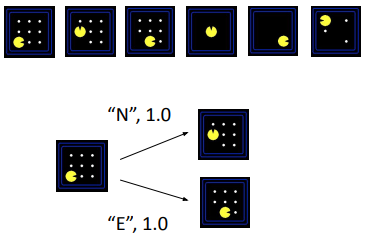
\includegraphics[height=2.7cm]{pacman.png}\\[0.2em]
      \scriptsize \keyword{Pacman}: position + food; move N/E/S/W
      \vspace{0.5em}\\
      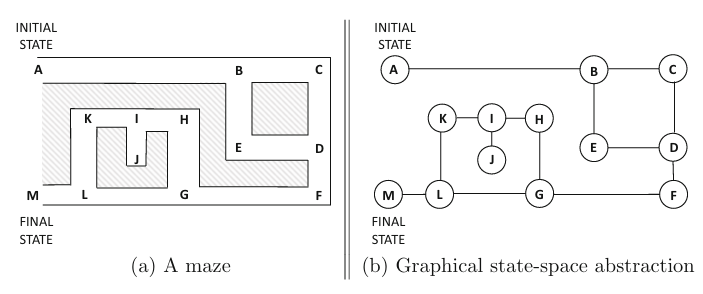
\includegraphics[height=2.6cm]{maze.png}\\[0.2em]
      \scriptsize \keyword{Maze}: position; move in 4 directions
    \end{column}
    \begin{column}{0.5\textwidth}
      \centering
      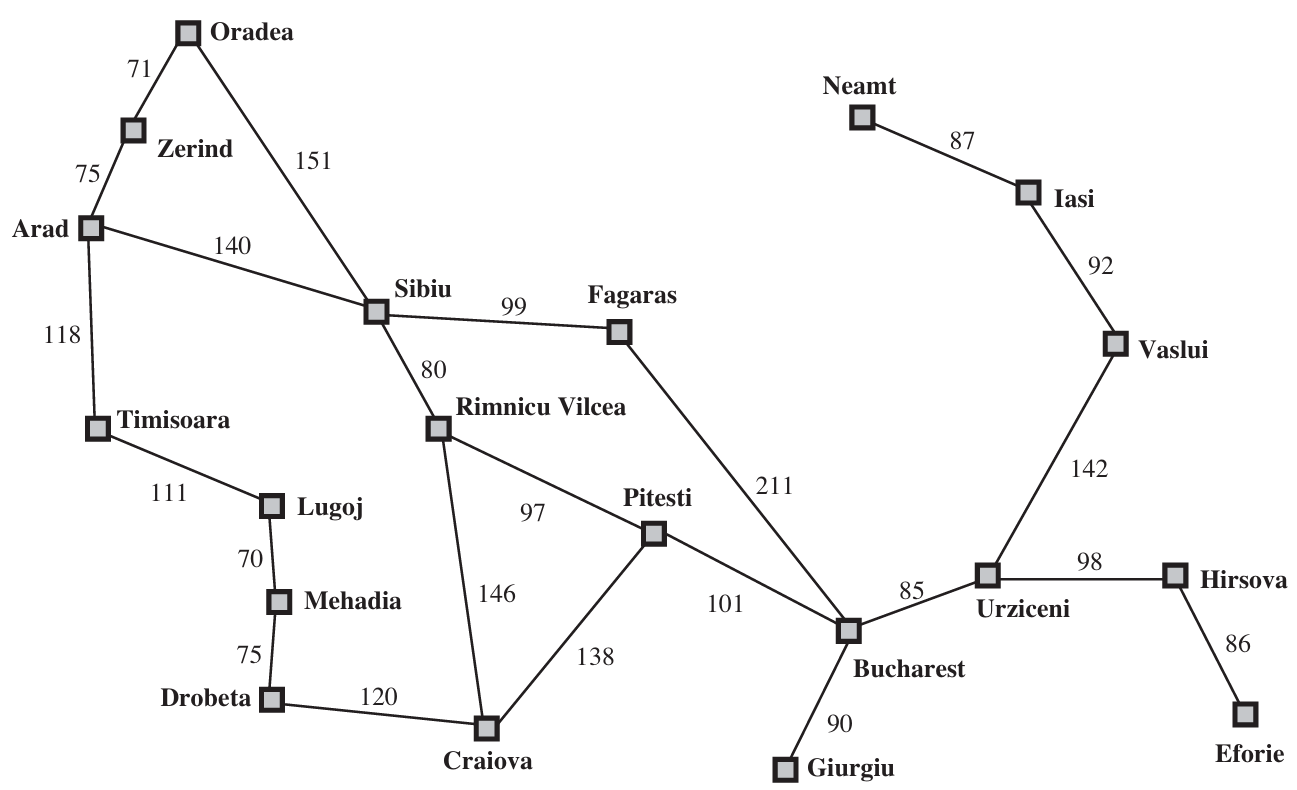
\includegraphics[width=\textwidth]{romania.png}\\[0.2em]
      \scriptsize \keyword{Romania}: current city; roads with distances;
      start Arad $\to$ goal Bucharest
    \end{column}
  \end{columns}
\end{frame}

% ============================================================
\section{Uninformed Search}
% ============================================================

\begin{frame}{Generic Search Framework}{One template, many strategies}
  \begin{columns}[T]
    \begin{column}{0.52\textwidth}
      \begin{block}{Components}
        \small
        \begin{itemize}
          \item \keyword{LIST} — frontier (nodes to explore)
          \item \keyword{VISIT} — already explored
          \item \keyword{pred} — predecessors for path recovery
          \item \keyword{Selection strategy} — defines the algorithm
        \end{itemize}
      \end{block}
      \centering\scriptsize
      FIFO $\Rightarrow$ BFS \quad LIFO $\Rightarrow$ DFS \quad
      priority $\Rightarrow$ UCS / A$^\ast$
    \end{column}
    \begin{column}{0.48\textwidth}
      \begin{center}
      \begin{tikzpicture}[node distance=0.42cm,
          b/.style={processstep, minimum width=4.2cm, minimum height=0.5cm}]
        \node[b, fill=SuccessGreen!20, draw=SuccessGreen] (i) {Init state $\to$ LIST};
        \node[b, below=of i] (sel) {Select node from LIST};
        \node[b, below=of sel] (goal) {Goal? $\Rightarrow$ return path};
        \node[b, below=of goal] (exp) {Expand: add neighbours};
        \draw[-{Latex[length=2mm]},PrimaryMid] (i)--(sel);
        \draw[-{Latex[length=2mm]},PrimaryMid] (sel)--(goal);
        \draw[-{Latex[length=2mm]},PrimaryMid] (goal)--(exp);
        \draw[-{Latex[length=2mm]},PrimaryMid] (exp.east) to[out=0,in=0] (sel.east);
      \end{tikzpicture}
      \end{center}
    \end{column}
  \end{columns}
\end{frame}

\begin{frame}{Breadth-First Search (BFS)}{Level-by-level, FIFO queue}
  \begin{columns}[T]
    \begin{column}{0.5\textwidth}
      Explores all nodes at depth $d$ before depth $d{+}1$.
      \begin{itemize}\small
        \item Insert at \keyword{end}, remove from \keyword{front} (FIFO)
        \item Finds the \keyword{shallowest} goal
      \end{itemize}
      \begin{exampleblock}{Good for}
        \small Shallow goals; optimal when all step costs are equal.
      \end{exampleblock}
      \begin{alertblock}{Cost}
        \small \important{Memory heavy} — stores the whole frontier.
      \end{alertblock}
    \end{column}
    \begin{column}{0.5\textwidth}
      \small
      \renewcommand{\arraystretch}{1.3}
      \begin{tabularx}{\linewidth}{@{}>{\bfseries}l >{\raggedright\arraybackslash}X@{}}
        \toprule
        \rowcolor{PrimaryDark}
        \textcolor{white}{Property} & \textcolor{white}{Value} \\
        \midrule
        Complete & Yes \\
        \rowcolor{PrimaryLight!25}
        Optimal & Yes$^\ast$ (equal costs) \\
        Time & $\mathcal{O}(b^{d})$ \\
        \rowcolor{PrimaryLight!25}
        Space & $\mathcal{O}(b^{d})$ \\
        \bottomrule
      \end{tabularx}
      \vspace{0.4em}
      \centering\scriptsize $b$: branching factor \quad $d$: depth of goal
    \end{column}
  \end{columns}
\end{frame}

\begin{frame}{Depth-First Search (DFS)}{Go deep, LIFO stack}
  \begin{columns}[T]
    \begin{column}{0.5\textwidth}
      Explores as deep as possible, then backtracks.
      \begin{itemize}\small
        \item Insert / remove at \keyword{end} (LIFO)
        \item Expands most recent node first
      \end{itemize}
      \begin{exampleblock}{Good for}
        \small Deep solutions, memory-limited settings.
      \end{exampleblock}
      \begin{alertblock}{Risk}
        \small Can loop forever (needs cycle detection); not optimal.
      \end{alertblock}
    \end{column}
    \begin{column}{0.5\textwidth}
      \small
      \renewcommand{\arraystretch}{1.3}
      \begin{tabularx}{\linewidth}{@{}>{\bfseries}l >{\raggedright\arraybackslash}X@{}}
        \toprule
        \rowcolor{PrimaryDark}
        \textcolor{white}{Property} & \textcolor{white}{Value} \\
        \midrule
        Complete & No (with cycles) \\
        \rowcolor{PrimaryLight!25}
        Optimal & No \\
        Time & $\mathcal{O}(b^{m})$ \\
        \rowcolor{PrimaryLight!25}
        Space & $\mathcal{O}(bm)$ \\
        \bottomrule
      \end{tabularx}
      \vspace{0.4em}
      \centering\scriptsize $m$: maximum depth of the tree
    \end{column}
  \end{columns}
\end{frame}

\begin{frame}{BFS vs.\ DFS}{Frontier shape trade-off}
  \begin{center}
    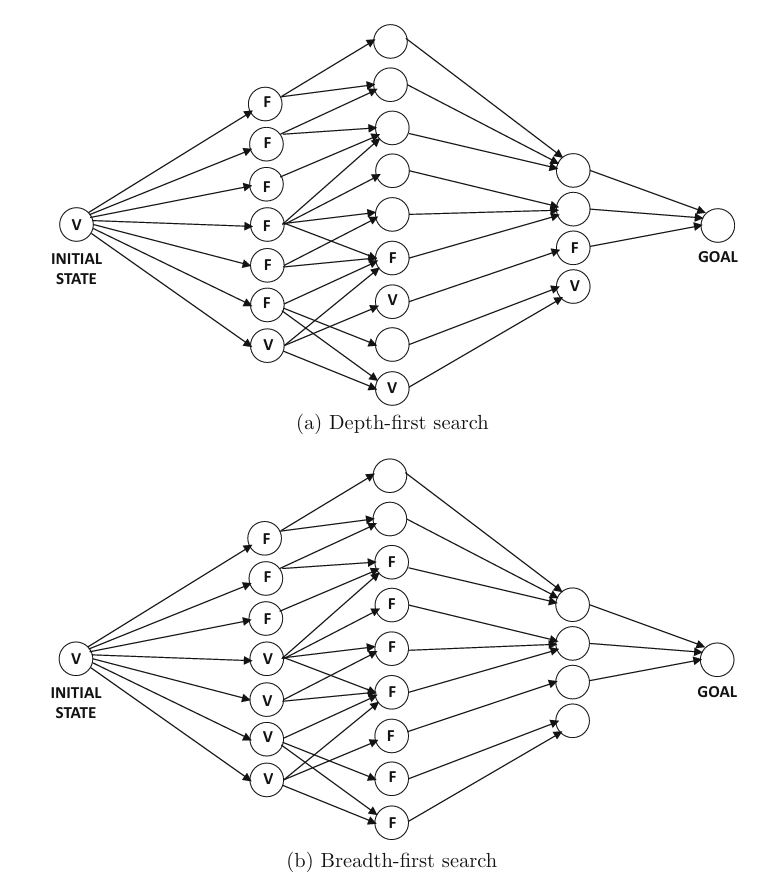
\includegraphics[width=0.82\textwidth]{bfsdfs.png}
  \end{center}
  \begin{center}\small
  \begin{tabular}{@{}lll@{}}
    \toprule
    \textbf{Aspect} & \textbf{BFS} & \textbf{DFS} \\
    \midrule
    Frontier & Wide, shallow & Deep, narrow \\
    Memory & $\mathcal{O}(b^{d})$ — high & $\mathcal{O}(bm)$ — low \\
    Optimal / Complete & Yes / Yes & No / No (cycles) \\
    \bottomrule
  \end{tabular}
  \end{center}
\end{frame}

\begin{frame}{Uniform-Cost Search (UCS)}{BFS for weighted graphs}
  \begin{columns}[T]
    \begin{column}{0.55\textwidth}
      Expand the node with the \keyword{lowest path cost} $g(n)$.
      \begin{itemize}\small
        \item Priority queue ordered by $g(n)$
        \item $g(n) = $ sum of edge costs from start
        \item Optimal for any non-negative costs
      \end{itemize}
      \begin{block}{Complexity}
        \small $\mathcal{O}\!\left(b^{\,C^{\ast}/\varepsilon}\right)$ time and space,
        where $C^{\ast}$ is the optimal cost and $\varepsilon$ the minimum edge cost.
      \end{block}
      \centering\scriptsize UCS $\equiv$ BFS when all edge costs are equal.
    \end{column}
    \begin{column}{0.45\textwidth}
      \begin{center}
      \begin{tikzpicture}[node distance=0.6cm and 0.9cm,
          st/.style={circle, draw=PrimaryMid, fill=PrimaryLight!45,
            minimum size=0.65cm, font=\small}, every edge quotes/.style={font=\scriptsize, auto}]
        \node[st, fill=AccentYellow!40, draw=AccentOrange] (s) {S};
        \node[st, below left=of s] (p) {p};
        \node[st, below=1.3cm of s] (e) {e};
        \node[st, below right=of e] (f) {f};
        \node[st, fill=SuccessGreen!35, draw=SuccessGreen, right=of f] (g) {G};
        \draw[-{Latex[length=1.6mm]},PrimaryMid] (s) to["1"] (p);
        \draw[-{Latex[length=1.6mm]},PrimaryMid] (p) to["2"] (e);
        \draw[-{Latex[length=1.6mm]},PrimaryMid] (e) to["2"] (f);
        \draw[-{Latex[length=1.6mm]},PrimaryMid] (f) to["1"] (g);
      \end{tikzpicture}\\
      \scriptsize Cheapest-first expansion order
      \end{center}
    \end{column}
  \end{columns}
\end{frame}

\begin{frame}{Bidirectional Search}{Meet in the middle}
  \begin{columns}[c]
    \begin{column}{0.5\textwidth}
      Run two searches: \keyword{forward} from start and \keyword{backward}
      from goal; stop when they meet.
      \vspace{0.4em}
      \begin{block}{Speed-up}
        \small
        $\mathcal{O}(b^{d}) \;\to\; \mathcal{O}\!\left(b^{d/2}\right)$
        \[ b{=}10,\, d{=}6:\ 10^{6} \to 2\times10^{3} \]
      \end{block}
    \end{column}
    \begin{column}{0.5\textwidth}
      \begin{center}
      \begin{tikzpicture}[node distance=1.1cm,
          b/.style={rounded corners=3pt, draw, minimum width=1.9cm,
            minimum height=0.8cm, font=\small\bfseries, align=center}]
        \node[b, fill=SuccessGreen!25, draw=SuccessGreen] (s) {Start};
        \node[b, fill=AccentYellow!35, draw=AccentOrange, right=of s] (m) {Meet};
        \node[b, fill=AlertRed!18, draw=AlertRed, right=of m] (g) {Goal};
        \draw[-{Latex[length=2mm]},PrimaryMid,thick] (s)--(m) node[midway,above,font=\scriptsize]{fwd};
        \draw[-{Latex[length=2mm]},PrimaryMid,thick] (g)--(m) node[midway,above,font=\scriptsize]{bwd};
      \end{tikzpicture}
      \end{center}
      \centering\scriptsize
      Needs predecessors and a meeting test; goal must be explicit.
    \end{column}
  \end{columns}
\end{frame}

\begin{frame}{Uninformed Search: Summary}{Choose by structure and resources}
  \small
  \renewcommand{\arraystretch}{1.3}
  \begin{center}
  \begin{tabularx}{\textwidth}{@{}>{\bfseries}l cc >{\raggedright\arraybackslash}X >{\raggedright\arraybackslash}X@{}}
    \toprule
    \rowcolor{PrimaryDark}
    \textcolor{white}{Algorithm} & \textcolor{white}{Compl.} & \textcolor{white}{Opt.} &
    \textcolor{white}{Time} & \textcolor{white}{Space} \\
    \midrule
    BFS & Yes & Yes$^\ast$ & $\mathcal{O}(b^{d})$ & $\mathcal{O}(b^{d})$ \\
    \rowcolor{PrimaryLight!25}
    DFS & No & No & $\mathcal{O}(b^{m})$ & $\mathcal{O}(bm)$ \\
    UCS & Yes & Yes & $\mathcal{O}(b^{C^{\ast}/\varepsilon})$ & $\mathcal{O}(b^{C^{\ast}/\varepsilon})$ \\
    \rowcolor{PrimaryLight!25}
    Bidirectional & Yes & Yes$^\ast$ & $\mathcal{O}(b^{d/2})$ & $\mathcal{O}(b^{d/2})$ \\
    \bottomrule
  \end{tabularx}
  \end{center}
  \begin{center}\small
    \important{Key takeaway:} uninformed search is inefficient for large spaces
    $\Rightarrow$ use \keyword{informed search}.
  \end{center}
\end{frame}

% ============================================================
\section{Informed Search}
% ============================================================

\begin{frame}{Heuristics}{Using knowledge to guide search}
  \begin{columns}[T]
    \begin{column}{0.5\textwidth}
      A \keyword{heuristic} $h(n)$ estimates the cost from $n$ to the nearest goal.
      \vspace{0.3em}
      \begin{block}{Evaluation functions}
        \small
        \begin{itemize}
          \item $g(n)$ — actual cost start $\to n$
          \item $h(n)$ — estimated cost $n \to$ goal
          \item $f(n)$ — estimated total through $n$
        \end{itemize}
      \end{block}
    \end{column}
    \begin{column}{0.5\textwidth}
      \begin{exampleblock}{Key properties}
        \small
        \begin{itemize}
          \item \keyword{Admissible}: $h(n) \le h^{\ast}(n)$ \\ (never overestimates)
          \item \keyword{Consistent}: $h(n) \le c(n,n') + h(n')$
        \end{itemize}
      \end{exampleblock}
      \centering\scriptsize Consistency $\Rightarrow$ admissibility (not vice versa).
      \vspace{0.4em}\\
      \scriptsize 8-puzzle: misplaced tiles, or sum of Manhattan distances.
    \end{column}
  \end{columns}
\end{frame}

\begin{frame}{Greedy Best-First Search}{$f(n) = h(n)$}
  \begin{columns}[T]
    \begin{column}{0.5\textwidth}
      Expand the node that \emph{appears} closest to the goal.
      \begin{itemize}\small
        \item Priority queue ordered by $h(n)$
        \item Ignores the cost already paid, $g(n)$
        \item Fast, but \important{not optimal / not complete}
      \end{itemize}
      \begin{block}{Typical heuristics}
        \scriptsize straight-line distance \textbullet\ Manhattan distance
        \textbullet\ misplaced tiles
      \end{block}
    \end{column}
    \begin{column}{0.5\textwidth}
      \begin{center}
      \begin{tikzpicture}[node distance=0.55cm and 0.9cm,
          st/.style={circle, draw=PrimaryMid, fill=PrimaryLight!45,
            minimum size=0.85cm, font=\scriptsize, align=center}]
        \node[st, fill=AccentYellow!40, draw=AccentOrange] (s) {S\\h=6};
        \node[st, below=of s] (a) {a\\h=5};
        \node[st, below left=of a] (d) {d\\h=2};
        \node[st, below right=of a] (e) {e\\h=1};
        \node[st, fill=SuccessGreen!35, draw=SuccessGreen, below=1.4cm of a] (g) {G\\h=0};
        \draw[-{Latex[length=1.6mm]},PrimaryMid] (s)--(a) node[midway,right,font=\scriptsize]{1};
        \draw[-{Latex[length=1.6mm]},PrimaryMid] (a)--(d) node[midway,left,font=\scriptsize]{3};
        \draw[-{Latex[length=1.6mm]},PrimaryMid] (a)--(e) node[midway,right,font=\scriptsize]{8};
        \draw[-{Latex[length=1.6mm]},PrimaryMid] (d)--(g) node[midway,left,font=\scriptsize]{2};
      \end{tikzpicture}\\
      \scriptsize Follows smallest $h$: S $\to$ a $\to$ d $\to$ G
      \end{center}
    \end{column}
  \end{columns}
\end{frame}

\begin{frame}{A$^\ast$ Search}{$f(n) = g(n) + h(n)$}
  \begin{columns}[T]
    \begin{column}{0.52\textwidth}
      The most widely used informed search: balances cost \keyword{paid}
      and cost \keyword{remaining}.
      \[ f(n) = \underbrace{g(n)}_{\text{start}\to n} + \underbrace{h(n)}_{n\to\text{goal}} \]
      \begin{itemize}\small
        \item Priority queue ordered by $f(n)$
        \item Expands the most promising \emph{total-cost} node
      \end{itemize}
      \begin{exampleblock}{Optimally efficient}
        \small With a given admissible $h$, no optimal algorithm expands fewer nodes.
      \end{exampleblock}
    \end{column}
    \begin{column}{0.48\textwidth}
      \begin{center}
      \begin{tikzpicture}[node distance=0.55cm and 0.7cm,
          st/.style={circle, draw=PrimaryMid, fill=PrimaryLight!45,
            minimum size=0.95cm, font=\scriptsize, align=center}]
        \node[st, fill=AccentYellow!40, draw=AccentOrange] (s) {S\\0+6};
        \node[st, below=of s] (a) {a\\1+5};
        \node[st, below left=of a] (d) {d\\4+2};
        \node[st, below right=of a] (e) {e\\9+1};
        \node[st, fill=SuccessGreen!35, draw=SuccessGreen, below=1.5cm of a] (g) {G\\6+0};
        \draw[-{Latex[length=1.6mm]},PrimaryMid] (s)--(a);
        \draw[-{Latex[length=1.6mm]},PrimaryMid] (a)--(d);
        \draw[-{Latex[length=1.6mm]},PrimaryMid] (a)--(e);
        \draw[-{Latex[length=1.6mm]},PrimaryMid] (d)--(g);
      \end{tikzpicture}\\
      \scriptsize Optimal path S$\to$a$\to$d$\to$G, $f=6$
      \end{center}
    \end{column}
  \end{columns}
\end{frame}

\begin{frame}{Why A$^\ast$ is Optimal}{Admissibility guarantees optimality}
  \begin{columns}[T]
    \begin{column}{0.55\textwidth}
      \begin{block}{Proof sketch}
        \small
        Suppose A$^\ast$ returned suboptimal $G_2$ (cost $C_2$), while optimal $G$
        has cost $C^{\ast} < C_2$. Some node $n$ on the optimal path is unexpanded.
        Since $h$ is admissible:
        \[ f(n) = g(n)+h(n) \le g(n)+h^{\ast}(n) = C^{\ast} < C_2 = f(G_2). \]
        A$^\ast$ expands by increasing $f$, so $n$ precedes $G_2$ — contradiction. $\blacksquare$
      \end{block}
    \end{column}
    \begin{column}{0.45\textwidth}
      \begin{alertblock}{Terminate correctly}
        \small Stop when the goal is \keyword{selected for expansion},
        not when first generated — otherwise the path may be suboptimal.
      \end{alertblock}
      \begin{block}{Condition}
        \small Optimal \emph{iff} $h$ is \keyword{admissible}
        (never overestimates the true cost).
      \end{block}
    \end{column}
  \end{columns}
\end{frame}

\begin{frame}{Designing Heuristics}{Better heuristics expand fewer nodes}
  \begin{columns}[T]
    \begin{column}{0.52\textwidth}
      \textbf{8-Puzzle heuristics}
      \begin{itemize}\small
        \item $h_1$ = number of \keyword{misplaced tiles}
        \item $h_2 = \sum_{\text{tiles}} |{\Delta x}| + |{\Delta y}|$ \\ (\keyword{Manhattan distance})
      \end{itemize}
      Both admissible; $h_2$ \keyword{dominates} $h_1$.
      \vspace{0.4em}
      \begin{block}{Techniques}
        \scriptsize
        Relaxed problems \textbullet\ pattern databases \textbullet\ learning
      \end{block}
    \end{column}
    \begin{column}{0.48\textwidth}
      \small
      \renewcommand{\arraystretch}{1.3}
      \begin{tabularx}{\linewidth}{@{}>{\raggedright\arraybackslash}X >{\raggedright\arraybackslash}X@{}}
        \toprule
        \rowcolor{PrimaryDark}
        \textcolor{white}{Heuristic} & \textcolor{white}{Avg nodes} \\
        \midrule
        None (UCS) & $\sim$170{,}000 \\
        \rowcolor{PrimaryLight!25}
        Misplaced $h_1$ & $\sim$500 \\
        Manhattan $h_2$ & $\sim$50 \\
        \bottomrule
      \end{tabularx}
      \vspace{0.4em}
      \centering\scriptsize Good $h$: admissible, consistent, accurate, fast.
    \end{column}
  \end{columns}
\end{frame}

% ============================================================
\section{Local Search}
% ============================================================

\begin{frame}{Local Search}{When only the final state matters}
  \begin{columns}[T]
    \begin{column}{0.5\textwidth}
      Explore the \keyword{neighborhood} of the current state; keep no path.
      \begin{itemize}\small
        \item State-centric loss functions
        \item Incremental refinement
        \item Low memory
      \end{itemize}
    \end{column}
    \begin{column}{0.5\textwidth}
      \begin{exampleblock}{Ideal for}
        \small 8-queens, TSP, scheduling, VLSI layout, vehicle routing —
        the \emph{result} matters, not the route to it.
      \end{exampleblock}
    \end{column}
  \end{columns}
\end{frame}

\begin{frame}{Hill Climbing}{Greedy local improvement}
  \begin{columns}[T]
    \begin{column}{0.48\textwidth}
      Repeatedly move to the best neighbor until none improves.
      \begin{itemize}\small
        \item 8-queens: move a queen to cut attacking pairs
        \item TSP: swap two cities to shorten the tour
      \end{itemize}
      \begin{alertblock}{Gets stuck at}
        \small local maxima \textbullet\ plateaus \textbullet\ ridges
      \end{alertblock}
      \scriptsize \keyword{Fixes:} random restart, stochastic / first-choice moves.
    \end{column}
    \begin{column}{0.52\textwidth}
      \begin{center}
      \begin{tikzpicture}
        \begin{axis}[width=6.2cm, height=4.2cm, tick style={draw=none},
          xtick=\empty, ytick=\empty, axis lines=left, clip=false,
          xlabel=\scriptsize state, ylabel=\scriptsize value, ymin=-1.4, ymax=2.2, xmin=0, xmax=10]
          \addplot[PrimaryMid, thick, samples=200, domain=0:10]
            {sin(deg(x)) + 0.6*sin(deg(2*x)) + 0.3*x*0.15};
          \node[font=\scriptsize, AlertRed] at (axis cs:1.7,1.7) {local max};
          \node[font=\scriptsize, SuccessGreen] at (axis cs:7.9,2.05) {global max};
          \node[font=\scriptsize, AccentOrange] at (axis cs:5.0,-0.9) {plateau/ridge};
        \end{axis}
      \end{tikzpicture}
      \end{center}
    \end{column}
  \end{columns}
\end{frame}

\begin{frame}{Simulated Annealing}{Accept some bad moves to escape optima}
  \begin{columns}[T]
    \begin{column}{0.55\textwidth}
      Inspired by metallurgical annealing: allow occasional \keyword{uphill} moves.
      \[ P(\text{accept}) = \begin{cases} 1 & \Delta L < 0 \\ e^{-\Delta L / T} & \Delta L \ge 0 \end{cases} \]
      \begin{itemize}\small
        \item High $T$: explore widely (accept bad moves often)
        \item Low $T$: exploit; $T \to 0$ becomes hill climbing
        \item Keep the \keyword{best} solution seen
      \end{itemize}
    \end{column}
    \begin{column}{0.45\textwidth}
      \begin{block}{Cooling schedules}
        \small
        \begin{itemize}
          \item Linear: $T_0 - \alpha t$
          \item Exponential: $T_0\,\gamma^{t}$
          \item Logarithmic: $T_0 / \log t$
        \end{itemize}
      \end{block}
      \centering\scriptsize
      \cmark\ escapes local optima \quad \xmark\ needs schedule tuning
    \end{column}
  \end{columns}
\end{frame}

\begin{frame}{Tabu Search}{Memory to avoid cycling}
  \begin{columns}[T]
    \begin{column}{0.55\textwidth}
      Enhance hill climbing with a \keyword{tabu list} of recently visited
      moves/states that are temporarily forbidden.
      \begin{itemize}\small
        \item \keyword{Tabu list}: fixed-size recent-move memory
        \item \keyword{Aspiration}: allow a tabu move if it beats the best-ever
        \item \keyword{Intensify} promising regions; \keyword{diversify} to new ones
      \end{itemize}
    \end{column}
    \begin{column}{0.45\textwidth}
      \begin{exampleblock}{Strengths}
        \small Escapes local optima deterministically; strong for TSP,
        scheduling, routing.
      \end{exampleblock}
      \centering\scriptsize Needs tuning of the tabu-list size.
    \end{column}
  \end{columns}
\end{frame}

\begin{frame}{Local Search: Comparison}{}
  \small
  \renewcommand{\arraystretch}{1.3}
  \begin{center}
  \begin{tabularx}{\textwidth}{@{}>{\bfseries}l >{\raggedright\arraybackslash}X >{\raggedright\arraybackslash}X >{\raggedright\arraybackslash}X@{}}
    \toprule
    \rowcolor{PrimaryDark}
    \textcolor{white}{Method} & \textcolor{white}{Escapes optima?} &
    \textcolor{white}{Memory} & \textcolor{white}{Best for} \\
    \midrule
    Hill Climbing & No & None & Simple, quick \\
    \rowcolor{PrimaryLight!25}
    Random Restart & Yes & None & Many local optima \\
    Simulated Annealing & Yes (prob.) & None & Large spaces \\
    \rowcolor{PrimaryLight!25}
    Tabu Search & Yes (determ.) & Tabu list & Avoiding cycles \\
    Genetic Algorithm & Yes & Population & Complex optimization \\
    \bottomrule
  \end{tabularx}
  \end{center}
\end{frame}

% ============================================================
\section{Genetic Algorithms}
% ============================================================

\begin{frame}{Genetic Algorithms}{Evolution as optimization}
  \begin{columns}[T]
    \begin{column}{0.5\textwidth}
      Evolve a \keyword{population} of solutions over generations.
      \begin{itemize}\small
        \item \keyword{Chromosome}: encoded solution
        \item \keyword{Fitness}: solution quality
        \item \keyword{Selection}: fitter parents reproduce
        \item \keyword{Crossover}: recombine parents
        \item \keyword{Mutation}: random diversity
      \end{itemize}
    \end{column}
    \begin{column}{0.5\textwidth}
      \begin{center}
      \begin{tikzpicture}[node distance=0.4cm,
          b/.style={processstep, minimum width=3.6cm, minimum height=0.5cm}]
        \node[b, fill=SuccessGreen!20, draw=SuccessGreen] (init) {Initialize population};
        \node[b, below=of init] (fit) {Evaluate fitness};
        \node[b, below=of fit] (sel) {Selection};
        \node[b, below=of sel] (cx) {Crossover};
        \node[b, below=of cx] (mut) {Mutation};
        \draw[-{Latex[length=1.6mm]},PrimaryMid] (init)--(fit);
        \draw[-{Latex[length=1.6mm]},PrimaryMid] (fit)--(sel);
        \draw[-{Latex[length=1.6mm]},PrimaryMid] (sel)--(cx);
        \draw[-{Latex[length=1.6mm]},PrimaryMid] (cx)--(mut);
        \draw[-{Latex[length=1.6mm]},PrimaryMid] (mut.east) to[out=0,in=0] (fit.east);
      \end{tikzpicture}
      \end{center}
    \end{column}
  \end{columns}
  \vspace{0.2em}
  \begin{center}\scriptsize
    \keyword{TSP example:} chromosome = city permutation; fitness = $-$tour length;
    order crossover; swap mutation.
  \end{center}
\end{frame}

% ============================================================
\section{Summary}
% ============================================================

\begin{frame}{Chapter Summary}{Key takeaways}
  \begin{columns}[T]
    \begin{column}{0.5\textwidth}
      \begin{block}{Uninformed}
        \small BFS (optimal, memory-heavy), DFS (light, not optimal),
        UCS (cost-optimal), bidirectional ($b^{d/2}$).
      \end{block}
      \begin{block}{Informed}
        \small Greedy ($h$) is fast but not optimal; A$^\ast$ ($g{+}h$) is optimal
        with an admissible heuristic.
      \end{block}
    \end{column}
    \begin{column}{0.5\textwidth}
      \begin{exampleblock}{Local \& evolutionary}
        \small Hill climbing, simulated annealing, tabu search, and genetic
        algorithms optimize the \emph{final state}.
      \end{exampleblock}
      \begin{alertblock}{Looking ahead}
        \small Ch.\,3: adversarial search and games (minimax, $\alpha$–$\beta$).
      \end{alertblock}
    \end{column}
  \end{columns}
\end{frame}

{\setbeamertemplate{footline}{}
\begin{frame}[plain,noframenumbering]
  \begin{tikzpicture}[remember picture,overlay]
    \fill[PrimaryDark](current page.north west) rectangle (current page.south east);
    \fill[PrimaryMid,opacity=0.35]
      ([shift={(0cm,-1.5cm)}]current page.north) circle(6.5cm);
  \end{tikzpicture}
  \vfill
  \begin{center}
    {\LARGE\textcolor{white}{\textbf{Thank you!}}}\\[0.6em]
    {\small\textcolor{PrimaryLight}{Questions \& Discussion}}\\[1.2em]
    {\footnotesize\textcolor{AccentYellow}{Next: Chapter 3 — Multiagent Search}}
  \end{center}
  \vfill
\end{frame}}

\end{document}
